\documentclass[aps,pra,onecolumn,11pt,tightenlines,notitlepage,nofootinbib]{revtex4-2}
\usepackage{amsmath,amssymb}
\usepackage{algorithm,algpseudocode}
\usepackage{tikz}
\usetikzlibrary{arrows.meta,shapes.geometric}
\usepackage[colorlinks=true,linkcolor=black,citecolor=black,urlcolor=blue]{hyperref}
\hypersetup{pdftitle={Gaussian orthant probabilities with BootLoops},pdfauthor={Implementation documentation}}
\newcommand{\dd}{\mathrm{d}}
\newcommand{\one}{\mathbf{1}}
\newcommand{\code}[1]{\texttt{\detokenize{#1}}}
\begin{document}
\raggedbottom
\title{Gaussian orthant probabilities with BootLoops}
\author{Implementation documentation}
\noaffiliation
\date{5 October 2026}
\begin{abstract}
The solver integrates a multivariate Gaussian density over regions defined
by coordinate bounds. These regions include orthants, finite boxes, and
boxes that extend to infinity in some directions. For general covariance
matrices, it connects the target integral to
an independent Gaussian integral, reduces its derivatives to a finite system
of boundary integrals, and uses BootLoops to transport that system. Two
structured matrix families instead admit one-dimensional quadrature. This
guide gives the reduction, the computational steps, and the main limits of
accuracy and dimension.
\end{abstract}
\maketitle

\section{Basic idea}
The idea of the solver is to convert an integral to a differential equation.
We introduce a parameter, differentiate the integral with respect to it,
and use integration by parts to eliminate the additional integrals that
appear. Known starting values then allow numerical evolution to the target.
A Gaussian half-line integral illustrates these steps:
\begin{equation}
 J(t)=\int_0^\infty e^{-x^2/2-tx}\dd x,
 \qquad J(0)=(\pi/2)^{1/2}.
 \label{eq:toy-integral}
\end{equation}
Differentiation gives $\frac{\dd J}{\dd t}=-M_1(t)$, where
$M_1(t)=\int_0^\infty x e^{-x^2/2-tx}\dd x$ is an unnormalized first
moment. To eliminate it, write $f_t(x)=e^{-x^2/2-tx}$ and integrate
$\partial f_t/\partial x=-(x+t)f_t$ over the half-line. The boundary values give
$f_t(\infty)-f_t(0)=-1=-M_1(t)-tJ(t)$, so $M_1(t)=1-tJ(t)$.
Substitution closes the equation:
\begin{equation}
 \frac{\dd J}{\dd t}=tJ(t)-1,\qquad J(0)=(\pi/2)^{1/2}.
 \label{eq:toy-equation}
\end{equation}
Solving this first-order ordinary differential equation yields the integral
at the desired parameter value. The constant term comes from the finite
boundary at $x=0$; the contribution at infinity vanishes.

This example varies a linear term in the exponent. The general solver
instead varies the coupling between Gaussian coordinates. It applies the
same reduction to the full integral and its boundary integrals, producing
a coupled first-order system that BootLoops evolves from known starting
values.

\section{Probability and continuation}
The integrals the solver actually evaluates are of course more complicated
than described above. Let $X$ have mean $\mu$ and positive-definite covariance
$\Sigma$. Set
$Q=\Sigma^{-1}$, $x=X-\mu$, $\ell=L-\mu$, and $u=U-\mu$. The target is
\begin{equation}
 p=\frac{(\det Q)^{1/2}}{(2\pi)^{d/2}}J_{\mathrm{full}}(1),\qquad
 J_{\mathrm{full}}(t)=\int_{\ell\leq x\leq u}
 \exp[-x^{\mathsf T}Q(t)x/2]\dd^d x .
 \label{eq:target}
\end{equation}
The inequalities apply coordinate by coordinate. Define
$D=\operatorname{diag}(Q)$ and $E=Q-D$, then set $Q(t)=D+tE$ for
$0\leq t\leq1$. At $t=0$ the integral factors into one-dimensional Gaussian
integrals; at $t=1$ it is the requested integral. The path remains valid
because $Q(t)=(1-t)D+tQ$ is positive definite. The solver transports
unnormalized integrals and applies the prefactor in Eq.~\eqref{eq:target}
only at the end.

This construction follows the integration-by-parts and differential-equation
strategy used for scattering integrals\cite{chetyrkin,kotikov,bootloops}.
The auxiliary mass flow method supplies another example of transport from a
tractable starting point\cite{amflow}. Here the independent Gaussian at
$t=0$ already supplies that point, so no auxiliary mass is needed.
Holonomic gradient methods apply related differential systems to Gaussian
orthant probabilities\cite{holonomic}.

\section{Boundary integrals and the differential system}
Differentiating $J_{\mathrm{full}}$ introduces Gaussian moments. The solver
eliminates them by integrating by parts and retaining integrals over finite
faces of the domain. A face $F$ leaves each coordinate free or fixes it at a
finite lower or upper endpoint; infinite endpoints contribute no boundary
term. If $A$ contains the free coordinates, $B$ the fixed coordinates, and
$b=x_B$, write
$J_F(t)=\int_{\ell_A}^{u_A}\exp[-x^{\mathsf T}Q(t)x/2]\dd x_A$.
These are density-slice integrals, not probabilities of landing on a face.

The reduction can be seen from one face. Put
$f_t=\exp[-x^{\mathsf T}Q(t)x/2]$,
$m_i=\int_F x_i f_t\dd x_A$, and
$M_{ij}=\int_F x_ix_j f_t\dd x_A$ for free indices. Direct differentiation
gives
\begin{equation}
 \frac{\dd J_F}{\dd t}=-\tfrac12\operatorname{tr}(E_{AA}M)
       -(E_{AB}b)^{\mathsf T}m
       -\tfrac12 b^{\mathsf T}E_{BB}b\,J_F .
 \label{eq:derivative}
\end{equation}
For a free coordinate $j$, let $\Delta_j$ be the upper child-face integral
minus the lower one, omitting infinite endpoints. Integrating
$\partial f_t/\partial x_j$ gives
$\Delta=-Q_{AA}(t)m-Q_{AB}(t)bJ_F$.
Integrating $\partial(x_i f_t)/\partial x_j$ similarly expresses $M$ in
terms of $J_F$, $m$, and child-face terms. A child face fixes one more
coordinate, so recursive reduction ends at corner values. Substitution
into Eq.~\eqref{eq:derivative} yields the closed system
\begin{equation}
 \frac{\dd J}{\dd t}=\mathcal A(t)J(t).
 \label{eq:system}
\end{equation}
Each entry of $\mathcal A(t)$ is rational: the inversions involve principal
submatrices of the linear matrix $Q(t)$. The retained family need not be a
minimal basis.

At $t=0$, a free coordinate $i$ contributes
$(2\pi/D_{ii})^{1/2}[\Phi(u_iD_{ii}^{1/2})-\Phi(\ell_iD_{ii}^{1/2})]$;
a coordinate fixed at $b_i$ contributes $\exp(-D_{ii}b_i^2/2)$.
Their product gives $s_F=J_F(0)$. Scaling by
$S=\operatorname{diag}(s_F)$ gives $W=S^{-1}J$ and
\begin{equation}
 \frac{\dd W}{\dd t}=\mathcal C(t)W,\qquad
 \mathcal C=S^{-1}\mathcal A S,\qquad W(0)=\one .
 \label{eq:scaled}
\end{equation}
BootLoops advances this rational system from $t=0$ to $t=1$ with local
Taylor expansions and step control. Finally,
$p=(\det Q)^{1/2}\,s_{\mathrm{full}}W_{\mathrm{full}}(1)/(2\pi)^{d/2}$.

\section{Implementation}
Algorithm~\ref{alg:general} states the general route. The independent and
two structured routes have separate entry points. The flow chart below
shows the numerical workflow and the role of each software component.
\begin{figure}[htbp]
\centering
\resizebox{\linewidth}{!}{%
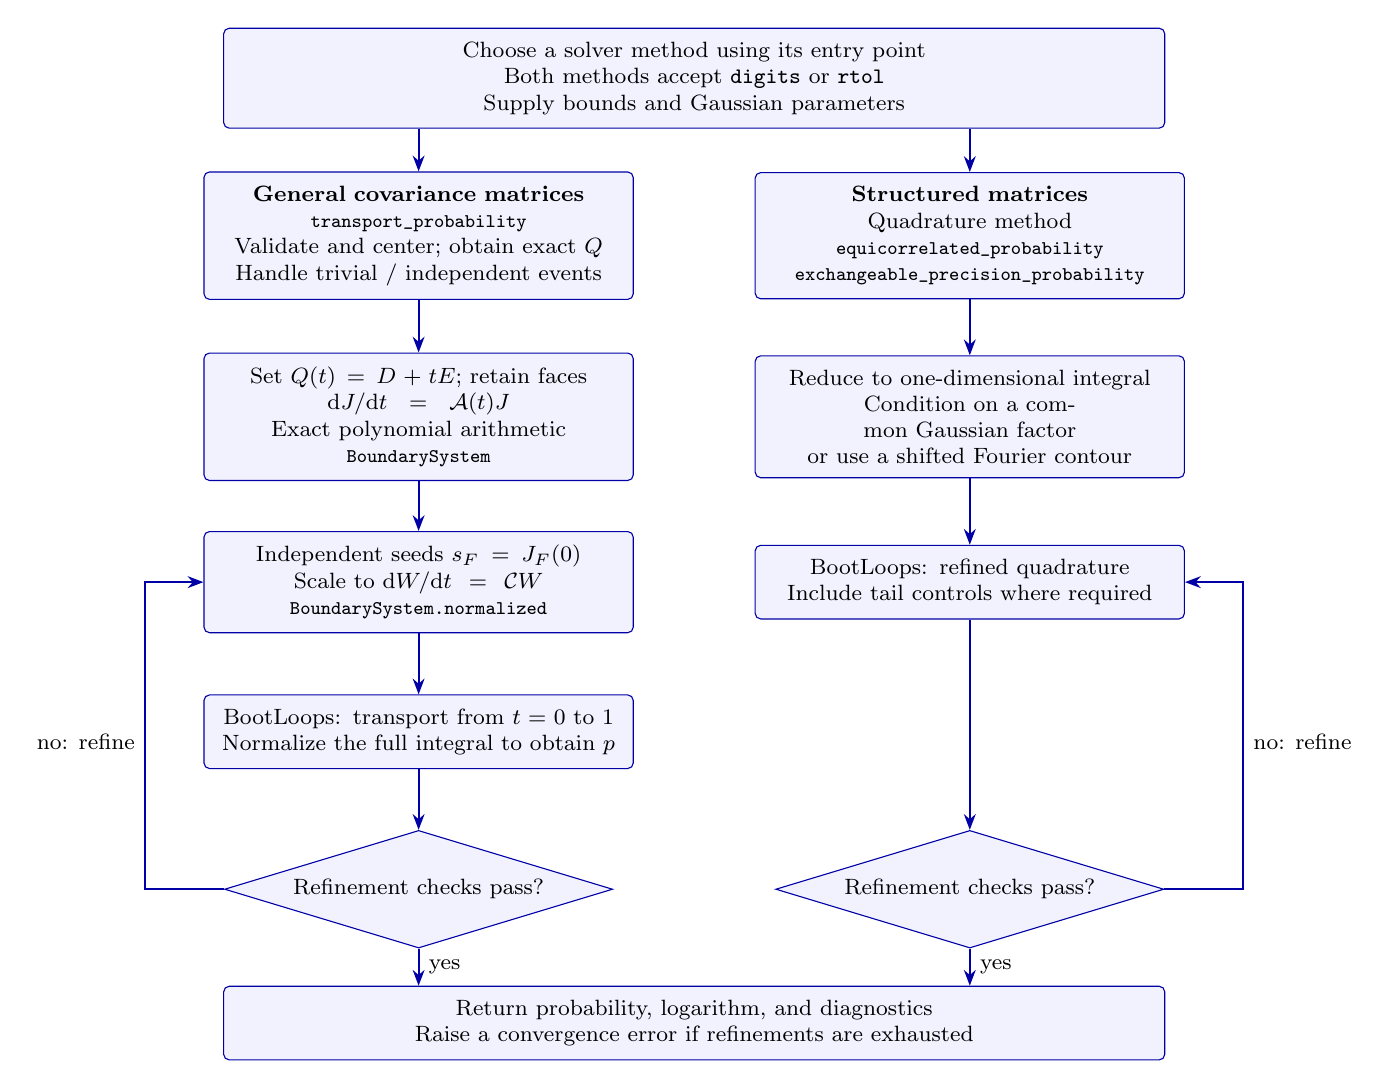
\begin{tikzpicture}[
    font=\footnotesize,
    process/.style={draw=blue!65!black, fill=blue!5, rounded corners=2pt,
        align=center, text width=5.1cm, minimum height=0.82cm, inner sep=5pt},
    decision/.style={draw=blue!65!black, fill=blue!5, diamond, aspect=3.3,
        align=center, inner sep=2pt, text width=3.5cm},
    flow/.style={-{Stealth[length=2mm]}, thick, draw=blue!65!black}
]
\node[process, text width=11.6cm] (input) at (3.5,0)
    {Choose a solver method using its entry point\\
     Both methods accept \code{digits} or \code{rtol}\\
     Supply bounds and Gaussian parameters};
\node[process] (prepare) at (0,-2.0)
    {\textbf{General covariance matrices}\\
     {\scriptsize\code{transport_probability}}\\
     Validate and center; obtain exact $Q$\\
     Handle trivial / independent events};
\node[process] (build) at (0,-4.3)
    {Set $Q(t)=D+tE$; retain faces\\
     $\dd J/\dd t=\mathcal A(t)J$\\
     Exact polynomial arithmetic\\
     {\scriptsize\code{BoundarySystem}}};
\node[process] (seed) at (0,-6.4)
    {Independent seeds $s_F=J_F(0)$\\
     Scale to $\dd W/\dd t=\mathcal C W$\\
     {\scriptsize\code{BoundarySystem.normalized}}};
\node[process] (transport) at (0,-8.3)
    {BootLoops: transport from $t=0$ to $1$\\
     Normalize the full integral to obtain $p$};
\node[decision] (check) at (0,-10.3)
    {Refinement checks pass?};
\node[process] (special) at (7,-2.0)
    {\textbf{Structured matrices}\\
     Quadrature method\\
     {\scriptsize\code{equicorrelated_probability}}\\
     {\scriptsize\code{exchangeable_precision_probability}}};
\node[process] (reduce) at (7,-4.3)
    {Reduce to one-dimensional integral\\
     Condition on a common Gaussian factor\\
     or use a shifted Fourier contour};
\node[process] (quad) at (7,-6.4)
    {BootLoops: refined quadrature\\
     Include tail controls where required};
\node[decision] (qcheck) at (7,-10.3)
    {Refinement checks pass?};
\node[process, text width=11.6cm] (result) at (3.5,-12.0)
    {Return probability, logarithm, and diagnostics\\
     Raise a convergence error if refinements are exhausted};
\draw[flow] (input.south -| prepare.north) -- (prepare.north);
\draw[flow] (input.south -| special.north) -- (special.north);
\draw[flow] (prepare) -- (build);
\draw[flow] (build) -- (seed);
\draw[flow] (seed) -- (transport);
\draw[flow] (transport) -- (check);
\draw[flow] (special) -- (reduce);
\draw[flow] (reduce) -- (quad);
\draw[flow] (quad) -- (qcheck);
\draw[flow] (check.south) -- node[right]{yes} (check.south |- result.north);
\draw[flow] (qcheck.south) -- node[right]{yes} (qcheck.south |- result.north);
\draw[flow] (check.west) -- ++(-1.0,0)
    |- node[pos=0.24, left, align=right]{no: refine} (seed.west);
\draw[flow] (qcheck.east) -- ++(1.0,0)
    |- node[pos=0.24, right, align=left]{no: refine} (quad.east);
\end{tikzpicture}%
}
\end{figure}
\begin{algorithm}[H]
\caption{General Gaussian box or orthant probability}
\label{alg:general}
\begin{algorithmic}[1]
\Require Bounds $L,U$; mean $\mu$; covariance $\Sigma$ or precision $Q$; \code{digits} or \code{rtol}
\Ensure Probability, logarithm, and diagnostics
\State Validate and center the inputs; obtain exact precision $Q$.
\If{the event is empty, full, or independent}
    \State \Return the corresponding direct result.
\EndIf
\State Set $Q(t)\gets\operatorname{diag}(Q)+t[Q-\operatorname{diag}(Q)]$.
\State Count and retain eligible faces, merging symmetric ones when possible.
\State Build the rational system $\dd J/\dd t=\mathcal A J$ by integration by parts.
\For{each permitted precision and transport refinement}
    \State Evaluate seeds $s_F=J_F(0)$ and form $\mathcal C=S^{-1}\mathcal A S$.
    \State Use BootLoops to transport $\dd W/\dd t=\mathcal C W$, $W(0)=\one$, to $t=1$.
    \State Normalize the full-region component to obtain $p$.
    \If{successive refinements and residual checks pass}
        \State \Return $p$, $\log p$, and diagnostics.
    \EndIf
\EndFor
\State Raise a convergence error.
\end{algorithmic}
\end{algorithm}

SymPy converts supplied decimal strings and fractions to exact rational
inputs, centers the bounds, and constructs the precision matrix and its
determinant\cite{sympy}. The Python connection builder uses SymPy rational
expressions; an optional compiled polynomial backend performs the same face
reduction with rational polynomial arithmetic. BootLoops evaluates the
system numerically. The adapter passes sparse rational coefficients and
estimated pole locations to its transport engine. Poles cannot lie on the
real path because all principal submatrices of $Q(t)$ remain positive
definite; nearby complex poles may still restrict step sizes.

As a check, take the positive quadrant in two dimensions with
$Q(t)=\left(\begin{smallmatrix}1&tc\\tc&1\end{smallmatrix}\right)$.
The full integral starts at $J(0)=\pi/2$; its edge and corner integrals
also have elementary starting values. Integration by parts gives a rational
differential system. With $c=-1/2$, the final covariance has correlation
$1/2$, and transport followed by Gaussian normalization gives $p=1/3$,
rather than the independent value $1/4$.

\section{Structured cases, accuracy, and limits}
Two matrix families avoid the face system. For equal nonnegative correlation
$\rho$ and common standardized bounds $\ell,u$, write
$X_i=\rho^{1/2}\,Z+(1-\rho)^{1/2}\,Z_i$ with independent standard-normal
variables. Conditioning on $Z=z$ gives the one-dimensional integral
$p=\int_{\mathbb R}\phi(z)g(z)^d\dd z$, where
$g(z)=\Phi[(u-\rho^{1/2}z)/(1-\rho)^{1/2}]
-\Phi[(\ell-\rho^{1/2}z)/(1-\rho)^{1/2}]$.
For exchangeable precision $Q=aI+b\one\one^{\mathsf T}$ with $b\geq0$
and common finite bounds, a Fourier identity separates the quadratic
coupling into one integration variable\cite{hubbard}. The implementation
shifts and scales that contour to reduce oscillation. BootLoops performs
refined one-dimensional quadrature for both families. These reductions do
not extend to arbitrary covariance matrices.

The interfaces accept either \code{digits} or \code{rtol}. The first asks
for a significant-digit representation; the second targets a relative
probability error and starts with cheaper settings. Both compare results
at increased working precision and tighter numerical controls. Agreement
provides evidence of accuracy, not a proof that every reported digit is
correct. Unlike Botev's minimax tilting estimator, which has sampling
uncertainty\cite{botev}, the solver uses deterministic refinements; neither
method acquires ground truth from its own error estimate.

For a general orthant the face system has up to $2^d$ states; a fully
bounded box has up to $3^d$. The default 256-state cap therefore limits
unstructured problems to eight one-sided or five fully bounded coordinates.
Symmetry can merge faces, but it does not remove the generic exponential
growth. High-dimensional results from the structured one-dimensional
functions should not be read as performance for general covariance matrices.

\begin{thebibliography}{9}
\bibitem{bootloops} M. Schwartz, \emph{BootLoops: an LLM-driven toolkit for exact quantitative science}, supplied manuscript (2026), Sec.~3.2; \href{https://bootloops.ai/BootLoops.pdf}{manuscript}.
\bibitem{chetyrkin} K. G. Chetyrkin and F. V. Tkachov, Nucl. Phys. B \textbf{192}, 159 (1981).
\bibitem{kotikov} A. V. Kotikov, Phys. Lett. B \textbf{254}, 158 (1991).
\bibitem{amflow} X. Liu and Y.-Q. Ma, Comput. Phys. Commun. \textbf{283}, 108565 (2023); \href{https://arxiv.org/abs/2201.11669}{arXiv:2201.11669}.
\bibitem{holonomic} T. Koyama and A. Takemura, \emph{Calculation of orthant probabilities by the holonomic gradient method} (2012); \href{https://arxiv.org/abs/1211.6822}{arXiv:1211.6822}.
\bibitem{sympy} A. Meurer \emph{et al.}, PeerJ Comput. Sci. \textbf{3}, e103 (2017).
\bibitem{hubbard} J. Hubbard, Phys. Rev. Lett. \textbf{3}, 77 (1959).
\bibitem{botev} Z. I. Botev, J. R. Stat. Soc. B \textbf{79}, 125 (2017); \href{https://arxiv.org/abs/1603.04166}{arXiv:1603.04166}.
\end{thebibliography}
\end{document}
